\documentclass[border=4pt]{standalone}
\usepackage{tikz}
\usetikzlibrary{arrows.meta}

\begin{document}
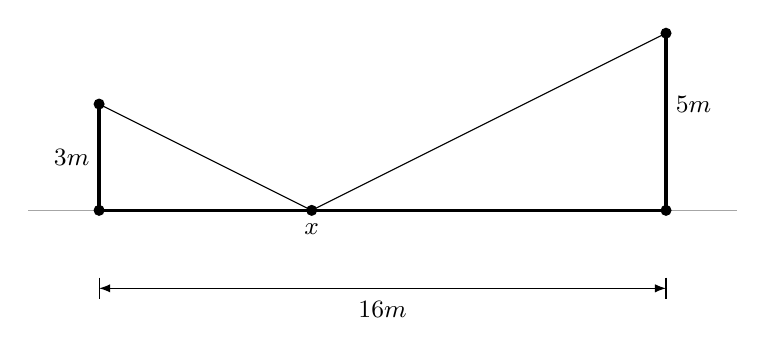
\begin{tikzpicture}[x=0.45cm, y=0.45cm, font=\small]
    \draw[gray!70] (-2,0) -- (18,0);
    \draw[line width=1.2pt] (0,0) -- (0,3);
    \draw[line width=1.2pt] (16,0) -- (16,5);
    \draw[line width=1.2pt] (0,0) -- (16,0);
    \draw (0,3) -- (6,0) -- (16,5);
    \foreach \p in {(0,0),(0,3),(16,0),(16,5),(6,0)} \fill \p circle (2pt);
    \node[left] at (0,1.5) {$3m$};
    \node[right] at (16,3) {$5m$};
    \node[below] at (6,-0.1) {$x$};
    \draw[{Latex[length=4pt]}-{Latex[length=4pt]}] (0,-2.2) -- (16,-2.2);
    \draw (0,-1.9) -- (0,-2.5); \draw (16,-1.9) -- (16,-2.5);
    \node[below] at (8,-2.3) {$16m$};
\end{tikzpicture}
\end{document}
